%Chap 5 pag 5
\definecolor{Purple}{RGB}{153,0,153}
\definecolor{Pink}{RGB}{255,0,131}
\begin{frame}{Ejemplo: colorear el mapa continuación}
\begin{figure}
    \centering
    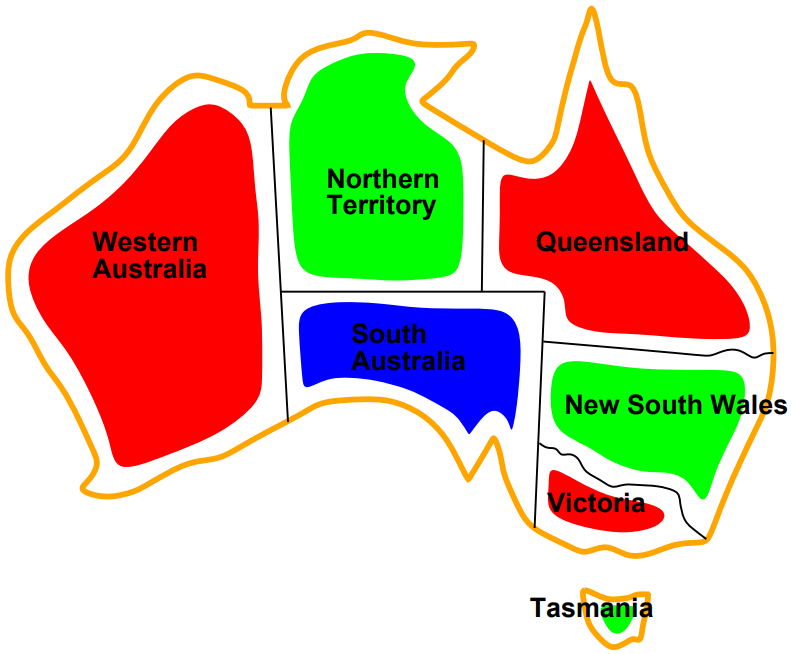
\includegraphics[width = 45mm, scale = 1]{images/5_5image.PNG}
\end{figure}
Las soluciones son tareas que satisfacen todas las restricciones, por ejemplo,\\
\scriptsize\textcolor{Purple}{ \left\lbrace WA = rojo, NT = verde, Q = rojo, NSW = verde, V = rojo, SA = azul, T = verde\right\rbrace}\
\end{frame}